% Created 2015-04-19 dom 15:49
\documentclass[xcolor={usenames,svgnames,dvipsnames}]{beamer}
\usepackage[utf8]{inputenc}
\usepackage[T1]{fontenc}
\usepackage{fixltx2e}
\usepackage{graphicx}
\usepackage{longtable}
\usepackage{float}
\usepackage{wrapfig}
\usepackage{rotating}
\usepackage[normalem]{ulem}
\usepackage{amsmath}
\usepackage{textcomp}
\usepackage{marvosym}
\usepackage{wasysym}
\usepackage{amssymb}
\usepackage{hyperref}
\tolerance=1000
\usepackage{color}
\usepackage{listings}
\AtBeginSubsection[]{\begin{frame}[plain]\tableofcontents[currentsubsection,sectionstyle=show/shaded,subsectionstyle=show/shaded/hide]\end{frame}}
\lstset{keywordstyle=\color{blue}, commentstyle=\color{gray!90}, basicstyle=\ttfamily\small, columns=fullflexible, breaklines=true,linewidth=\textwidth, backgroundcolor=\color{gray!23}, basewidth={0.5em,0.4em}, literate={á}{{\'a}}1 {ñ}{{\~n}}1 {é}{{\'e}}1 {ó}{{\'o}}1 {º}{{\textordmasculine}}1}
\usepackage{mathpazo}
\hypersetup{colorlinks=true, linkcolor=Blue, urlcolor=Blue}
\usepackage{fancyvrb}
\DefineVerbatimEnvironment{verbatim}{Verbatim}{fontsize=\tiny, formatcom = {\color{black!70}}}
\usetheme{Goettingen}
\usecolortheme{rose}
\usefonttheme{serif}
\author{Oscar Perpiñán Lamigueiro \\ \url{http://oscarperpinan.github.io}}
\date{}
\title{Introducción a R}
\hypersetup{
  pdfkeywords={},
  pdfsubject={},
  pdfcreator={Emacs 24.4.1 (Org mode 8.2.7c)}}
\begin{document}

\maketitle

\section{Introducción}
\label{sec-1}
\subsection{¿Qué es \texttt{R}?}
\label{sec-1-1}
\begin{frame}[fragile,label=sec-1-1-1]{¿Qué es \texttt{R}?}
 Es un entorno de programación orientado al cálculo, manipulación de datos, y representación gráfica, publicado como software libre con licencia GNU-GPL.
\begin{center}
\url{http://www.R-project.org} 
\end{center}
\end{frame}

\begin{frame}[fragile,label=sec-1-1-2]{Para instalar \texttt{R}}
 \begin{itemize}
\item Windows: \url{http://cran.es.r-project.org/bin/windows/base/}
\item Mac: \url{http://cran.es.r-project.org/bin/macosx/}
\item Linux: \url{http://cran.es.r-project.org/bin/linux/}
\end{itemize}
\end{frame}

\begin{frame}[label=sec-1-1-3]{Interfaces para R}
\begin{itemize}
\item En mi opinión, la mejor interfaz para R es \href{http://ess.r-project.org/}{ESS} con \href{http://www.gnu.org/software/emacs/}{Emacs}.
\item Para los que prefieren una interfaz gráfica es recomendable \href{http://www.rstudio.com/ide/}{RStudio}:
\begin{itemize}
\item Instalador: \url{http://www.rstudio.com/ide/download/desktop}
\item Introducción: \url{http://www.rstudio.com/ide/docs/using/source}
\end{itemize}
\end{itemize}
\end{frame}



\begin{frame}[label=sec-1-1-4]{R está muy bien documentado}
\begin{itemize}
\item \href{http://cran.r-project.org/manuals.html}{Manuales Oficiales}

\begin{itemize}
\item \href{http://cran.r-project.org/doc/manuals/r-release/R-intro.html}{Introduction to R}

\item \href{http://cran.r-project.org/doc/manuals/r-release/R-data.html}{R Data Import/Export}

\item \href{http://cran.r-project.org/doc/manuals/r-release/R-admin.html}{R Installation and Administration}

\item \href{http://cran.r-project.org/doc/manuals/r-release/R-exts.html}{Writing R Extensions}

\item \href{http://cran.r-project.org/doc/manuals/r-release/R-lang.html}{R language definition}

\item \href{http://cran.r-project.org/doc/manuals/r-release/R-ints.html}{R Internals}
\end{itemize}

\item \href{http://cran.r-project.org/other-docs.html}{Manuales externos}
\end{itemize}
\end{frame}

\begin{frame}[label=sec-1-1-5]{Otros recursos de información}
\begin{itemize}
\item \href{http://www.r-project.org/mail.html}{Listas de correo} (sin olvidar respetar \href{http://www.r-project.org/posting-guide.html}{estos consejos})
\begin{itemize}
\item Generales: R-announce, R-help, R-devel
\item Special Interest Group (SIG) mailing lists
\end{itemize}
\item \href{http://www.r-bloggers.com}{R-bloggers}
\item \href{http://stackoverflow.com/questions/tagged/r}{stackoverflow}
\end{itemize}
\end{frame}

\begin{frame}[label=sec-1-1-6]{R es un proyecto colaborativo}
\begin{itemize}
\item Una de las grandes riquezas de R es la cantidad de paquetes (más
de 6000 actualmente) que amplían sus funcionalidades.
\item La lista completa está en \url{http://cran.es.r-project.org/web/packages/}.
\item Las CRAN Task Views agrupan por temáticas:
\url{http://cran.r-project.org/web/views/}
\end{itemize}
\end{frame}

\begin{frame}[fragile,label=sec-1-1-7]{Más de 6000 paquetes disponibles}
 \begin{itemize}
\item Algunos vienen instalados y se cargan al empezar:
\end{itemize}
\lstset{language=R,label= ,caption= ,numbers=none}
\begin{lstlisting}
  sessionInfo()
\end{lstlisting}
\end{frame}
\begin{frame}[fragile,label=sec-1-1-8]{Más de 6000 paquetes disponibles}
 \begin{itemize}
\item Otros vienen instalados pero hay que cargarlos:
\end{itemize}
\lstset{language=R,label= ,caption= ,numbers=none}
\begin{lstlisting}
  library(lattice)
  packageVersion('lattice')
\end{lstlisting}
\lstset{language=R,label= ,caption= ,numbers=none}
\begin{lstlisting}
  packageDescription('lattice')
\end{lstlisting}
\end{frame}

\begin{frame}[fragile,label=sec-1-1-9]{Más de 6000 paquetes disponibles}
 \begin{itemize}
\item Otros hay que instalarlos y después cargarlos:
\end{itemize}
\lstset{language=R,label= ,caption= ,numbers=none}
\begin{lstlisting}
  install.packages('data.table')
  library('data.table')
  packageDescription('data.table')
\end{lstlisting}
\end{frame}


\subsection{Guía para usar el curso}
\label{sec-1-2}

\begin{frame}[label=sec-1-2-1]{Interfaz gráfica: RStudio}
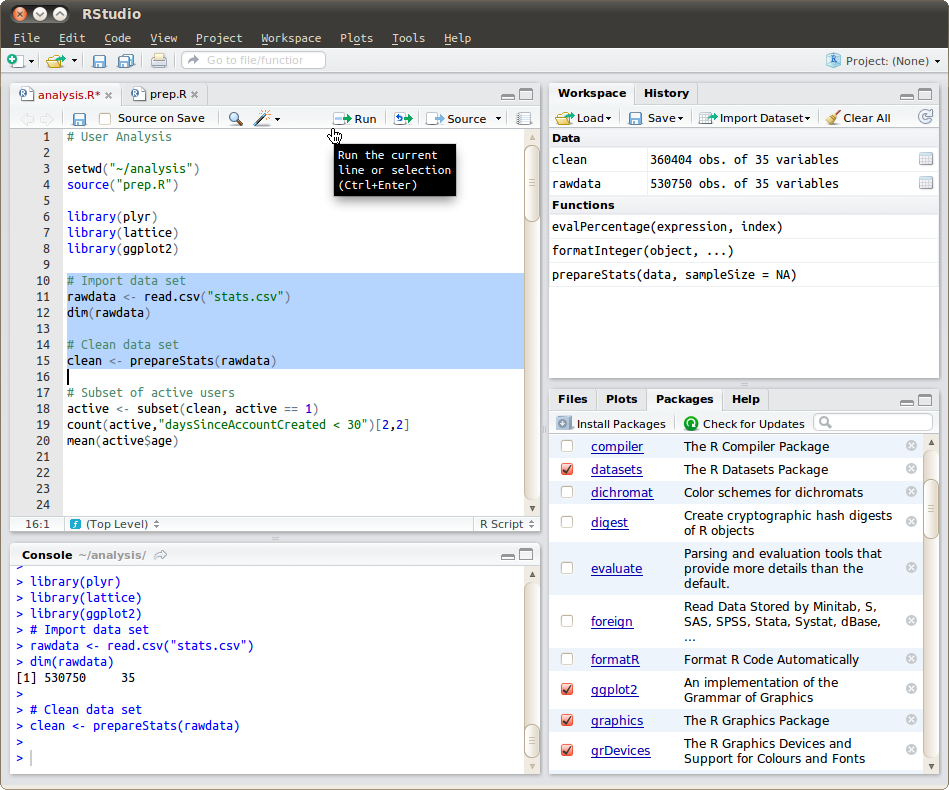
\includegraphics[width=.9\linewidth]{figs/rstudio-ubuntu.png}
\end{frame}

\begin{frame}[fragile,label=sec-1-2-2]{Interfaz gráfica: RStudio}
 \begin{itemize}
\item La consola de R es el área en la que se ejecuta código (\texttt{Ctrl + 2})
\begin{itemize}
\item Indica con \texttt{>} que está listo para aceptar comandos.
\item Indica con \texttt{+} que está a la espera de completar comando (salir con \texttt{Esc}).
\item Permite recuperar comandos antiguos con flechas arriba y abajo.
\end{itemize}
\item El área de código es donde se edita y almacena código (\texttt{Ctrl + 1})
\begin{itemize}
\item Escribir (y grabar) en área de código y enviar a consola (\texttt{Ctrl + Enter})
\item Permite completar comandos con \texttt{TAB}
\end{itemize}
\item Para la asignación \texttt{<-} usar \texttt{Alt + -}
\end{itemize}
\end{frame}

\begin{frame}[fragile,label=sec-1-2-3]{Material}
 \begin{itemize}
\item Primero obtenemos una copia local del repositorio. Opciones:

\begin{itemize}
\item Descargando el repositorio en formato ZIP: descomprímelo en una ruta sencilla (por ejemplo, en Windows \texttt{C:\textbackslash{}cursoR\textbackslash{}} y en Linux/Mac \texttt{/home/miusuario/cursoR/}).

\item Usando \texttt{git}:
\end{itemize}
\end{itemize}
\lstset{language=sh,label= ,caption= ,numbers=none}
\begin{lstlisting}
git clone git://github.com/oscarperpinan/intro.git
\end{lstlisting}
\end{frame}

\begin{frame}[fragile,label=sec-1-2-4]{Material}
 \begin{itemize}
\item Todo el código del curso asume que la ruta de trabajo coincide con la carpeta local: definimos la ruta de trabajo con \texttt{setwd}
\end{itemize}
\lstset{language=R,label= ,caption= ,numbers=none}
\begin{lstlisting}
setwd('/ruta/de/copia/local/del/repositorio/')
\end{lstlisting}

\begin{itemize}
\item Comprobamos que todo ha ido bien. El resultado de la siguiente instrucción debe ser la estructura de carpetas y ficheros del repositorio:
\end{itemize}
\lstset{language=R,label= ,caption= ,numbers=none}
\begin{lstlisting}
dir()
\end{lstlisting}
\end{frame}

\begin{frame}[fragile,label=sec-1-2-5]{Material}
 \begin{itemize}
\item Finalmente hay que instalar los paquetes que se emplean a lo largo del curso. Algunos ya vendrán instalados con tu distribución de R por ser paquetes recomendados. En la siguiente instrucción usamos el \emph{CRAN mirror} de la Oficina de Software Libre (CIXUG).
\end{itemize}
\lstset{language=R,label= ,caption= ,numbers=none}
\begin{lstlisting}
install.packages(c('lattice', 'latticeExtra', 'RColorBrewer',
                   'zoo', 'reshape2', 'ggplot2'),
                 repos = 'http://ftp.cixug.es/CRAN')
\end{lstlisting}
\end{frame}

\begin{frame}[label=sec-1-2-6]{Bloc de Notas}
\begin{itemize}
\item Usaremos un bloc de notas colaborativo para escribir código juntos y resolver dudas. Está accesible en: \url{https://etsidifv.titanpad.com/r-ice-upm}

\item La clave será comunicada al inicio de las clases.
\end{itemize}
\end{frame}


\section{Vectores y Matrices}
\label{sec-2}

\subsection{Vectores}
\label{sec-2-1}
\begin{frame}[fragile,label=sec-2-1-1]{Primeros pasos}
 \lstset{language=R,label= ,caption= ,numbers=none}
\begin{lstlisting}
x <- 1
x
length(x)
class(x)

x <- c(1, 2, 3)
x
length(x)
class(x)
\end{lstlisting}
\end{frame}

\begin{frame}[fragile,label=sec-2-1-2]{Primeras funciones}
 \lstset{language=R,label= ,caption= ,numbers=none}
\begin{lstlisting}
class(c)
class(length)
length
\end{lstlisting}
\end{frame}

\begin{frame}[fragile,label=sec-2-1-3]{Operaciones sencillas con vectores}
 \lstset{language=R,label= ,caption= ,numbers=none}
\begin{lstlisting}
  x + 1
  y <- 1:10
  x + y
  x * y
  x^2
  x^2 + y^3
  exp(x)
  log(x)
\end{lstlisting}
\end{frame}

\begin{frame}[fragile,label=sec-2-1-4]{¿Y qué hago cuando necesito ayuda?}
 \lstset{language=R,label= ,caption= ,numbers=none}
\begin{lstlisting}
help(exp)
help(log)
\end{lstlisting}
\end{frame}

\begin{frame}[fragile,label=sec-2-1-5]{Generar vectores con \texttt{seq}}
 \lstset{language=R,label= ,caption= ,numbers=none}
\begin{lstlisting}
x1 <- seq(1, 100, by=2)
x1
help(seq)

seq(1, 100, 10)
seq(1, 100, length=10)
seq(1, 1, 10)

x <- seq(1, 100, length=10)
x
length(x)

x <- seq(1, 100, length=10)
y <- seq(2, 100, length=50)
\end{lstlisting}
\end{frame}

\begin{frame}[fragile,label=sec-2-1-6]{Unir vectores con \texttt{c}}
 \lstset{language=R,label= ,caption= ,numbers=none}
\begin{lstlisting}
z <- c(x, y)
z
z + c(1, 2)
z + c(1, 2, 3, 4, 5, 6, 7)
z <- c(z, z, z, z)
z
\end{lstlisting}
\end{frame}

\begin{frame}[fragile,label=sec-2-1-7]{Generar vectores con \texttt{rep}}
 \lstset{language=R,label= ,caption= ,numbers=none}
\begin{lstlisting}
rep(1:10, 4)

length(z)

rep(c(1, 2, 3), 10)
rep(c(1, 2, 3), each=10)
help(rep)
\end{lstlisting}
\end{frame}


\begin{frame}[fragile,label=sec-2-1-8]{Indexado numérico de vectores}
 \lstset{language=R,label= ,caption= ,numbers=none}
\begin{lstlisting}
  x <- seq(1, 100, 2)
  1:5
  x[c(1, 2, 3, 4, 5)]
  x[1:5]
  x[10:5]
\end{lstlisting}
\end{frame}

\begin{frame}[fragile,label=sec-2-1-9]{Indexado de vectores con condiciones lógicas}
 \lstset{language=R,label= ,caption= ,numbers=none}
\begin{lstlisting}
  condicion <- (x>30)
  condicion
  class(condicion)
\end{lstlisting}
\end{frame}

\begin{frame}[fragile,label=sec-2-1-10]{Indexado de vectores con condiciones lógicas}
 \lstset{language=R,label= ,caption= ,numbers=none}
\begin{lstlisting}
  x==37
  x[x==37]
  x[x!=9]
  x[x>20]
\end{lstlisting}

\begin{itemize}
\item Y aquí ¿qué ocurre?
\end{itemize}
\lstset{language=R,label= ,caption= ,numbers=none}
\begin{lstlisting}
  x[x=10]
\end{lstlisting}
\end{frame}

\begin{frame}[fragile,label=sec-2-1-11]{Indexado de vectores con \texttt{\%in\%}}
 \lstset{language=R,label= ,caption= ,numbers=none}
\begin{lstlisting}
y <- seq(101, 200, 2)
y %in% c(101, 127, 141)
y
y[y %in% c(101, 127, 141)]
\end{lstlisting}
\end{frame}

\begin{frame}[fragile,label=sec-2-1-12]{Indexado de vectores con condiciones múltiples}
 \lstset{language=R,label= ,caption= ,numbers=none}
\begin{lstlisting}
z <- c(x, y)
z
z>150
z[z>150]
z[z<30 | z>150]
z[z>=30 & z<=150]
z[c(1, 10, 40, 80)]
\end{lstlisting}
\end{frame}

\begin{frame}[fragile,label=sec-2-1-13]{Indexado de vectores con condiciones múltiples}
 \lstset{language=R,label= ,caption= ,numbers=none}
\begin{lstlisting}
cond  <-  (x>10) & (x<50)
cond
cond  <-  (x>=10) & (x<=50)
cond
x[cond]
\end{lstlisting}
\end{frame}

\begin{frame}[fragile,label=sec-2-1-14]{Con las condiciones se pueden hacer operaciones}
 \lstset{language=R,label= ,caption= ,numbers=none}
\begin{lstlisting}
sum(cond)
!cond
sum(!cond)
length(x[cond])
length(x[!cond])
as.numeric(cond)
\end{lstlisting}
\end{frame}


\begin{frame}[fragile,label=sec-2-1-15]{Funciones predefinidas}
 \lstset{language=R,label= ,caption= ,numbers=none}
\begin{lstlisting}
summary(x)
mean(x)
sd(x)
median(x)
max(x)
min(x)
range(x)
quantile(x)
\end{lstlisting}
\end{frame}



\subsection{Matrices}
\label{sec-2-2}
\begin{frame}[fragile,label=sec-2-2-1]{Construir una matriz}
 \lstset{language=R,label= ,caption= ,numbers=none}
\begin{lstlisting}
  z <- 1:12
  M  <-  matrix(z, nrow=3)
  M
  z
  help(matrix)
  class(M)
  dim(M)
  summary(M)
\end{lstlisting}
\end{frame}

\begin{frame}[fragile,label=sec-2-2-2]{Matrices a partir de vectores: \texttt{rbind} y \texttt{cbind}}
 \lstset{language=R,label= ,caption= ,numbers=none}
\begin{lstlisting}
x <- 1:10
y <- 1:10
z <- 1:10
z <- y <- x <- 1:10

M <- cbind(x, y, z)
M
M <- rbind(x, y, z)
M

rbind(M, M)
cbind(M, M)
\end{lstlisting}
\end{frame}

\begin{frame}[fragile,label=sec-2-2-3]{Transponer una matriz}
 \lstset{language=R,label= ,caption= ,numbers=none}
\begin{lstlisting}
t(M)
class(t)
dim(t(M))
\end{lstlisting}
\end{frame}

\begin{frame}[fragile,label=sec-2-2-4]{Operaciones con matrices}
 \lstset{language=R,label= ,caption= ,numbers=none}
\begin{lstlisting}
M * M
M ^ 2
M %*% M
M %*% t(M)
help('%*%')
\end{lstlisting}
\end{frame}

\begin{frame}[fragile,label=sec-2-2-5]{Operaciones con matrices: funciones predefinidas}
 \lstset{language=R,label= ,caption= ,numbers=none}
\begin{lstlisting}
sum(M)
rowSums(M)
colSums(M)
rowMeans(M)
colMeans(M)
\end{lstlisting}
\end{frame}

\begin{frame}[fragile,label=sec-2-2-6]{La función \texttt{apply}}
 \lstset{language=R,label= ,caption= ,numbers=none}
\begin{lstlisting}
help(apply)
apply(M, 1, sum)
apply(M, 2, sum)
apply(M, 1, mean)
apply(M, 2, mean)
apply(M, 1, sd, na.rm=TRUE)
apply(M, 2, sd)
\end{lstlisting}
\end{frame}

\begin{frame}[fragile,label=sec-2-2-7]{\texttt{sweep}}
 \begin{itemize}
\item Usamos el conjunto de datos \texttt{state.x77}
\end{itemize}
\lstset{language=R,label= ,caption= ,numbers=none}
\begin{lstlisting}
  head(state.x77)
\end{lstlisting}
\begin{itemize}
\item Calculamos el máximo por columna
\end{itemize}
\lstset{language=R,label= ,caption= ,numbers=none}
\begin{lstlisting}
maxes <- apply(state.x77, 2, max)
\end{lstlisting}
\begin{itemize}
\item Dividimos cada columna por su máximo
\end{itemize}
\lstset{language=R,label= ,caption= ,numbers=none}
\begin{lstlisting}
  stateNorm <- sweep(state.x77, 2, maxes, FUN="/")
  head(stateNorm)
\end{lstlisting}
\end{frame}

\begin{frame}[fragile,label=sec-2-2-8]{Indexado de matrices}
 \lstset{language=R,label= ,caption= ,numbers=none}
\begin{lstlisting}
M
M[]
M[1, ]
M[, 1]
sum(M[, 1])
M[1:2, ]
M[1:2, 2:3]
M[1, c(1, 4)]
M[-1,]
M[-c(1, 2),]
\end{lstlisting}
\end{frame}


\subsection{Valores ausentes}
\label{sec-2-3}

\begin{frame}[fragile,label=sec-2-3-1]{¿Qué es \texttt{NA}?}
 \lstset{language=R,label= ,caption= ,numbers=none}
\begin{lstlisting}
  class(NA)
  x <- rnorm(100)
  idx <- sample(length(x), 10)
  idx
  x[idx]
  x2 <- x
  x2[idx] <- NA
  x2
\end{lstlisting}
\end{frame}

\begin{frame}[fragile,label=sec-2-3-2]{\texttt{NA} en las funciones}
 \lstset{language=R,label= ,caption= ,numbers=none}
\begin{lstlisting}
  summary(x)
  mean(x)
  sum(x)
  
  summary(x2)
  mean(x2)
  sum(x2)
\end{lstlisting}
\end{frame}

\begin{frame}[fragile,label=sec-2-3-3]{\texttt{NA} en las funciones}
 \lstset{language=R,label= ,caption= ,numbers=none}
\begin{lstlisting}
mean(x2, na.rm=TRUE)
sum(x2, na.rm=TRUE)
sd(x2, na.rm=TRUE)
class(TRUE)
\end{lstlisting}
\end{frame}


\section{Funciones}
\label{sec-3}

\subsection{Definición de funciones}
\label{sec-3-1}
\begin{frame}[fragile,label=sec-3-1-1]{Para definir una función usamos la función \texttt{function}}
 \lstset{language=R,label= ,caption= ,numbers=none}
\begin{lstlisting}
  myFun <- function(x, y) x + y
  myFun(3, 4)
  class(myFun)
\end{lstlisting}
\end{frame}

\begin{frame}[fragile,label=sec-3-1-2]{Definir una función a partir de funciones}
 \lstset{language=R,label= ,caption= ,numbers=none}
\begin{lstlisting}
foo  <-  function(x, ...){
  mx <- mean(x, ...)
  medx <- median(x, ...)
  sdx <- sd(x, ...)
  c(mx, medx, sdx)
  }
\end{lstlisting}
O en forma resumida:
\lstset{language=R,label= ,caption= ,numbers=none}
\begin{lstlisting}
foo <- function(x, ...){c(mean(x, ...), median(x, ...), sd(x, ...))}
\end{lstlisting}
\end{frame}


\subsection{Uso de funciones}
\label{sec-3-2}
\begin{frame}[fragile,label=sec-3-2-1]{Y ahora usamos la función con vectores}
 \lstset{language=R,label= ,caption= ,numbers=none}
\begin{lstlisting}
foo(1:10)

rnorm(100)
help(rnorm)
foo(rnorm(1e5))
\end{lstlisting}
\end{frame}

\begin{frame}[fragile,label=sec-3-2-2]{Y también funciona con matrices}
 \lstset{language=R,label= ,caption= ,numbers=none}
\begin{lstlisting}
rowMeans(M)
apply(M, 1, foo)
colMeans(M)
apply(M, 2, foo)
\end{lstlisting}
\end{frame}

\begin{frame}[fragile,label=sec-3-2-3]{La función \texttt{outer}}
 \lstset{language=R,label= ,caption= ,numbers=none}
\begin{lstlisting}
f <- function(x, y)x^2+y^2
f
f(1, 2)
x
y

z <- outer(x, y, f)
z
image(x, y, z)
\end{lstlisting}
\end{frame}


\section{Listas y data.frame}
\label{sec-4}

\subsection{Listas}
\label{sec-4-1}
\begin{frame}[fragile,label=sec-4-1-1]{Para crear una lista usamos la función \texttt{list}}
 \lstset{language=R,label= ,caption= ,numbers=none}
\begin{lstlisting}
  lista <- list(a=c(1,3,5),
                b=c('l', 'p', 'r', 's'),
                c=3)
  class(list)
  class(lista)
\end{lstlisting}
\end{frame}

\begin{frame}[fragile,label=sec-4-1-2]{Podemos acceder a los elementos\ldots{}}
 \begin{itemize}
\item Por su nombre
\end{itemize}
\lstset{language=R,label= ,caption= ,numbers=none}
\begin{lstlisting}
lista
lista$a
lista$b
lista$c
\end{lstlisting}

\begin{itemize}
\item o por su índice
\end{itemize}
\lstset{language=R,label= ,caption= ,numbers=none}
\begin{lstlisting}
  lista[1]
  lista[[1]]
  
  class(lista[1])
  class(lista[[1]])
  
  lista[2]
  lista[[2]]
  
  class(lista[2])
  class(lista[[2]])
\end{lstlisting}
\end{frame}

\begin{frame}[fragile,label=sec-4-1-3]{Cada elemento es diferente}
 \begin{itemize}
\item Clase
\end{itemize}
\lstset{language=R,label= ,caption= ,numbers=none}
\begin{lstlisting}
class(lista)
class(lista$a)
class(lista$b)
class(lista$c)
\end{lstlisting}
\begin{itemize}
\item Longitud
\end{itemize}
\lstset{language=R,label= ,caption= ,numbers=none}
\begin{lstlisting}
length(lista)
length(lista$a)
length(lista$b)
length(lista$c)
\end{lstlisting}
\end{frame}

\begin{frame}[fragile,label=sec-4-1-4]{Para matrices \texttt{apply}, para listas \texttt{lapply} y \texttt{sapply}}
 \lstset{language=R,label= ,caption= ,numbers=none}
\begin{lstlisting}
lapply(lista, length)
sapply(lista, length)

lista <- list(x = 1:10,
              y = seq(0, 10, 2),
              z = rnorm(30))
lista

lapply(lista, sum)
lapply(lista, median)
lapply(lista, foo)
\end{lstlisting}
\end{frame}


\subsection{Data.frame}
\label{sec-4-2}
\begin{frame}[fragile,label=sec-4-2-1]{Para crear un \texttt{data.frame}\ldots{}}
 \lstset{language=R,label= ,caption= ,numbers=none}
\begin{lstlisting}
  df <- data.frame(x = 1:10,
                   y = rnorm(10),
                   z = 0)
  
  length(df)
  dim(df)
\end{lstlisting}
\end{frame}
\begin{frame}[fragile,label=sec-4-2-2]{Podemos acceder a los elementos}
 \begin{itemize}
\item Por su nombre
\end{itemize}
\lstset{language=R,label= ,caption= ,numbers=none}
\begin{lstlisting}
df$x
df$y
df$z
\end{lstlisting}

\begin{itemize}
\item Por su índice
\end{itemize}
\lstset{language=R,label= ,caption= ,numbers=none}
\begin{lstlisting}
df
df[1,]
df[,1]
df[,2]
\end{lstlisting}
\end{frame}

\begin{frame}[fragile,label=sec-4-2-3]{La regla del reciclaje}
 \lstset{language=R,label= ,caption= ,numbers=none}
\begin{lstlisting}
  year <- 2011
  month <- 1:12
  class <- c('A', 'B', 'C')
  vals <- rnorm(12)
  
  dats <- data.frame(year, month, class, vals)
  dats
\end{lstlisting}
\end{frame}
\begin{frame}[fragile,label=sec-4-2-4]{La función \texttt{expand.grid}}
 \lstset{language=R,label= ,caption= ,numbers=none}
\begin{lstlisting}
  x <- y <- seq(-4*pi, 4*pi, len=200)
  df <- expand.grid(x = x, y = y)
  head(df)
  tail(df)
  summary(df)
  dim(df)
  names(df)
\end{lstlisting}
\end{frame}

\begin{frame}[fragile,label=sec-4-2-5]{Funciones sobre \texttt{data.frame}}
 \lstset{language=R,label= ,caption= ,numbers=none}
\begin{lstlisting}
  circles <- function(object){
    r <- with(object, sqrt(x^2 + y^2))
    res <- cos(r^2)*exp(-r/6)
    res}
  
  df$result <- circles(df)
  head(df)
\end{lstlisting}
\end{frame}

\begin{frame}[fragile,label=sec-4-2-6]{Una imagen vale más que mil palabras}
 \lstset{language=R,label= ,caption= ,numbers=none}
\begin{lstlisting}
  library(lattice)
  levelplot(result ~ x + y, data=df)
\end{lstlisting}
\end{frame}

\begin{frame}[fragile,label=sec-4-2-7]{Unir dos \texttt{data.frame}}
 \begin{itemize}
\item Primero construimos un \texttt{data.frame} de ejemplo
\end{itemize}
\lstset{language=R,label= ,caption= ,numbers=none}
\begin{lstlisting}
  USStates <- as.data.frame(state.x77)
  USStates$Name <- rownames(USStates)
  rownames(USStates) <- NULL
\end{lstlisting}
\begin{itemize}
\item Lo partimos en estados \guillemotleft{}fríos\guillemotright{} y estados \guillemotleft{}grandes\guillemotright{}
\end{itemize}
\lstset{language=R,label= ,caption= ,numbers=none}
\begin{lstlisting}
  coldStates <- USStates[USStates$Frost>150,
                         c('Name', 'Frost')]
  largeStates <- USStates[USStates$Area>1e5,
                          c('Name', 'Area')]
\end{lstlisting}
\begin{itemize}
\item Unimos los dos conjuntos (estados \guillemotleft{}fríos\guillemotright{} y \guillemotleft{}grandes\guillemotright{})
\end{itemize}
\lstset{language=R,label= ,caption= ,numbers=none}
\begin{lstlisting}
  merge(coldStates, largeStates)
\end{lstlisting}
\end{frame}

\begin{frame}[fragile,label=sec-4-2-8]{\texttt{merge} usa \texttt{match}}
 \begin{itemize}
\item Estados grandes que también son fríos
\end{itemize}
\lstset{language=R,label= ,caption= ,numbers=none}
\begin{lstlisting}
  idxLarge <- match(largeStates$Name,
                    coldStates$Name,
                    nomatch=0)
  idxLarge
  
  coldStates[idxLarge,]
\end{lstlisting}

\begin{itemize}
\item Estados frios que también son grandes
\end{itemize}
\lstset{language=R,label= ,caption= ,numbers=none}
\begin{lstlisting}
  idxCold <- match(coldStates$Name,
                   largeStates$Name,
                   nomatch=0)
  idxCold
  
  largeStates[idxCold,]
\end{lstlisting}
\end{frame}

\section{Factores, fechas y caracteres}
\label{sec-5}
\subsection{\texttt{factor}}
\label{sec-5-1}
\begin{frame}[fragile,label=sec-5-1-1]{Una variable numérica que nos servirá para el ejemplo}
 \lstset{language=R,label= ,caption= ,numbers=none}
\begin{lstlisting}
  N <- 100
  edad <- sample(seq(18, 40, 1), N, replace=TRUE)
  summary(edad)
\end{lstlisting}
\end{frame}

\begin{frame}[fragile,label=sec-5-1-2]{Una variable cualitativa se define con \texttt{factor}}
 \begin{itemize}
\item Ahora es un \texttt{character}
\end{itemize}
\lstset{language=R,label= ,caption= ,numbers=none}
\begin{lstlisting}
  sexo <- sample(c('H', 'M'), N, replace=TRUE)
  class(sexo)
  summary(sexo)
\end{lstlisting}
\begin{itemize}
\item Ahora es un \texttt{factor}
\end{itemize}
\lstset{language=R,label= ,caption= ,numbers=none}
\begin{lstlisting}
  sexo <- factor(sexo)
  class(sexo)
  summary(sexo)
  levels(sexo)
  nlevels(sexo)
\end{lstlisting}
\end{frame}

\begin{frame}[fragile,label=sec-5-1-3]{Los \texttt{factor} sirven para agrupar}
 \begin{itemize}
\item Con la función \texttt{table}
\end{itemize}
\lstset{language=R,label= ,caption= ,numbers=none}
\begin{lstlisting}
  table(edad, sexo)
  table(edad > 30, sexo)
  table(edad %in% 20:30, sexo)
\end{lstlisting}

\begin{itemize}
\item Con \texttt{tapply} o \texttt{aggregate}
\end{itemize}
\lstset{language=R,label= ,caption= ,numbers=none}
\begin{lstlisting}
tapply(edad,sexo, mean)
aggregate(edad ~ sexo, FUN=median)
\end{lstlisting}
\end{frame}

\begin{frame}[fragile,label=sec-5-1-4]{Los factores sirven para separar}
 \lstset{language=R,label= ,caption= ,numbers=none}
\begin{lstlisting}
  edadSexo <- split(edad, sexo)
  class(edadSexo)
  
  sapply(edadSexo, mean)
\end{lstlisting}
\end{frame}

\begin{frame}[fragile,label=sec-5-1-5]{Los \texttt{factor} se pueden generar a partir de variables numéricas}
 \begin{itemize}
\item Por ejemplo, con \texttt{cut}
\end{itemize}
\lstset{language=R,label= ,caption= ,numbers=none}
\begin{lstlisting}
  gEdad <- cut(edad, breaks=4)
  class(gEdad)
  levels(gEdad)
  nlevels(gEdad)
\end{lstlisting}

\begin{itemize}
\item Nuevamente \texttt{table}
\end{itemize}
\lstset{language=R,label= ,caption= ,numbers=none}
\begin{lstlisting}
  table(gEdad)
  table(gEdad, sexo)
\end{lstlisting}
\end{frame}

\subsection{Fechas}
\label{sec-5-2}

\begin{frame}[fragile,label=sec-5-2-1]{\texttt{Date}}
 \lstset{language=R,label= ,caption= ,numbers=none}
\begin{lstlisting}
  as.Date('2013-02-06')
  as.Date('2013/02/06')
  
  as.Date('06.02.2013')
  as.Date('06.02.2013', format='%d.%m.%Y')
  
  as.Date(37, origin='2013-01-01')
\end{lstlisting}
\end{frame}

\begin{frame}[fragile,label=sec-5-2-2]{Secuencias temporales con \texttt{Date}}
 \lstset{language=R,label= ,caption= ,numbers=none}
\begin{lstlisting}
  seq(as.Date('2004-01-01'), by='day', length=10)
  seq(as.Date('2004-01-01'), by='month', length=10)
  seq(as.Date('2004-01-01'), by='10 day', length=10)
\end{lstlisting}
\end{frame}

\begin{frame}[fragile,label=sec-5-2-3]{POSIXct}
 \lstset{language=R,label= ,caption= ,numbers=none}
\begin{lstlisting}
  as.POSIXct('2013-02-06')
  ISOdate(2013, 2, 7)
\end{lstlisting}

\lstset{language=R,label= ,caption= ,numbers=none}
\begin{lstlisting}
hoy <- as.POSIXct('2013-02-06')

help(format.POSIXct)
format(hoy, '%Y')
format(hoy, '%d')
format(hoy, '%m')
format(hoy, '%b')
format(hoy, '%d de %B de %Y')
\end{lstlisting}

\lstset{language=R,label= ,caption= ,numbers=none}
\begin{lstlisting}
  hora <- Sys.time()
  hora
  
  format(hora, '%H:%M:%S')
  format(hora, '%H horas, %M minutos y %S segundos')
\end{lstlisting}
\end{frame}

\begin{frame}[fragile,label=sec-5-2-4]{Secuencias temporales con \texttt{POSIXct}}
 \lstset{language=R,label= ,caption= ,numbers=none}
\begin{lstlisting}
seq(as.POSIXct('2004-01-01'), by='month', length=10)
seq(as.POSIXct('2004-01-01 10:00:00'), by='15 min', length=10)
\end{lstlisting}
\end{frame}

\begin{frame}[fragile,label=sec-5-2-5]{Zonas horarias}
 \lstset{language=R,label= ,caption= ,numbers=none}
\begin{lstlisting}
  as.POSIXct('2013-02-06 15:30:00',
             tz='GMT')
  as.POSIXct('2013-02-06 15:30:00',
             tz='Europe/Madrid')
\end{lstlisting}

\lstset{language=R,label= ,caption= ,numbers=none}
\begin{lstlisting}
hawaii <- as.POSIXct('2013-02-06 15:30:00', tz='HST')
## Character
format(hawaii, tz='GMT')
## POSIXct
as.POSIXct(format(hawaii, tz='GMT'), tz='GMT')
\end{lstlisting}
\end{frame}

\subsection{Caracteres}
\label{sec-5-3}

\begin{frame}[fragile,label=sec-5-3-1]{Bastan unas simples comillas}
 \lstset{language=R,label= ,caption= ,numbers=none}
\begin{lstlisting}
  cadena <- "Hola mundo"
  class(cadena)
  nchar(cadena)
\end{lstlisting}

\begin{itemize}
\item Y aquí, ¿qué pasa?
\end{itemize}
\lstset{language=R,label= ,caption= ,numbers=none}
\begin{lstlisting}
length(cadena)
cadena[1]
cadena[2]
\end{lstlisting}
\end{frame}

\begin{frame}[fragile,label=sec-5-3-2]{Un vector de \texttt{character}}
 \lstset{language=R,label= ,caption= ,numbers=none}
\begin{lstlisting}
  cadenaVec <- c("Hola mundo", "Hello world")
  nchar(cadenaVec)
  length(cadenaVec)
\end{lstlisting}
\end{frame}

\begin{frame}[fragile,label=sec-5-3-3]{Para mostrarlos usamos \texttt{cat} o \texttt{print}}
 \lstset{language=R,label= ,caption= ,numbers=none}
\begin{lstlisting}
  a = 2
  b = 3
  
  cat('La suma de', a, 'y', b, 'es', a + b)
  
  cat('La suma de', a, 'y', b, 'es', a + b, fill=TRUE)
  
  cat('La suma de', a, 'y', b, 'es', a + b, '\n',
      'La multiplicación de', a, 'por', b, 'es', a*b, '\n')
  
  cat('La suma de', a, 'y', b, 'es', a + b, '\n',
      'La multiplicación de', a, 'por', b, 'es', a*b, fill=15)
\end{lstlisting}
\end{frame}

\begin{frame}[fragile,label=sec-5-3-4]{Los \texttt{character} se pueden unir\ldots{}}
 \begin{itemize}
\item Primero sencillo
\end{itemize}
\lstset{language=R,label= ,caption= ,numbers=none}
\begin{lstlisting}
  paste('Hello', 'World', sep='_')
  
  paste(cadenaVec)
  paste(cadenaVec, collapse='=')
\end{lstlisting}
\begin{itemize}
\item Y algo más complicado
\end{itemize}
\lstset{language=R,label= ,caption= ,numbers=none}
\begin{lstlisting}
  paste('X', 1:5, sep='.')
  paste(c('A', 'B'), 1:5, sep='.')
  
  paste(c('A', 'B'), 1:5, sep='.', collapse='|')
\end{lstlisting}
\end{frame}

\begin{frame}[fragile,label=sec-5-3-5]{\ldots{} y también se pueden separar\ldots{}}
 \lstset{language=R,label= ,caption= ,numbers=none}
\begin{lstlisting}
  strsplit(cadenaVec, split=' ')
  strsplit(cadenaVec, split='')
\end{lstlisting}

\lstset{language=R,label= ,caption= ,numbers=none}
\begin{lstlisting}
  chSep <- strsplit(cadenaVec, split=' ')
  class(chSep)
  length(chSep)
  sapply(chSep, length)
  sapply(chSep, nchar)
\end{lstlisting}
\end{frame}

\begin{frame}[fragile,label=sec-5-3-6]{\ldots{} y, por supuesto, manipular}
 \lstset{language=R,label= ,caption= ,numbers=none}
\begin{lstlisting}
  sub('o', '0', 'Hola Mundo')
  gsub('o', '0', 'Hola Mundo')
  
  substring(cadena, 1) <- 'HOLA'
  cadena
  
  tolower(cadena)
  toupper(cadena)
\end{lstlisting}
\end{frame}



\section{Bucles y condiciones}
\label{sec-6}
\subsection{Bucles \texttt{for}}
\label{sec-6-1}
\begin{frame}[fragile,label=sec-6-1-1]{\texttt{for}}
 \lstset{language=R,label= ,caption= ,numbers=none}
\begin{lstlisting}
  for(n in c(2,5,10,20,50)) {
      x <- rnorm(n)
      cat(n,":", sum(x^2),"\n")
  }
\end{lstlisting}
\end{frame}
\subsection{Condiciones con \texttt{if}, \texttt{else} e \texttt{ifelse}}
\label{sec-6-2}
\begin{frame}[fragile,label=sec-6-2-1]{\texttt{if}}
 \lstset{language=R,label= ,caption= ,numbers=none}
\begin{lstlisting}
  x <- rnorm(10)
  x2 <- numeric(length(x))
  for (i in seq_along(x2)){
      if (x[i]<0) x2[i] <- 0 else x2[i] <- 1
      }
  cbind(x, x2)
\end{lstlisting}
\end{frame}
\begin{frame}[fragile,label=sec-6-2-2]{\texttt{ifelse}}
 \lstset{language=R,label= ,caption= ,numbers=none}
\begin{lstlisting}
  x <- rnorm(10)
  ifelse(x>0, 1, 0)
\end{lstlisting}
\end{frame}
% Emacs 24.4.1 (Org mode 8.2.7c)
\end{document}